\begin{figure}[t]
\centering
\ref{combined_legend}
\subfigure[
Accuracy plateaus due to \textit{attention's distractibility}.
]{
\begin{minipage}[t]{0.45\linewidth}
\centering
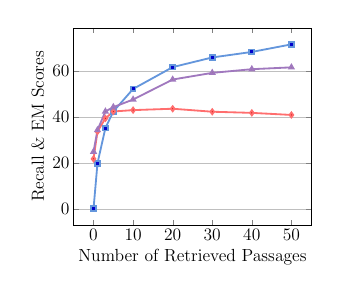
\begin{tikzpicture}[scale=0.44]
    \begin{axis}[
        xlabel=Number of Retrieved Passages,
        ylabel=Recall \& EM Scores,
        % y label style={at={(-0.00,0.5)}},
        ymajorgrids=true,
        font=\Large,
        legend style={at={(0.8,1.05)},anchor=south,legend columns=3,font={\fontsize{5pt}{5pt}\selectfont},/tikz/every even column/.append style={column sep=0.2cm}},
        legend to name=combined_legend
        ]
        \addplot+[color={rgb,255:red,100;green,150;blue,220},line width=1.5pt,mark=square*,mark size=2pt] coordinates {
            (0,0)
            (1,19.8)
            (3,35.1)
            (5,42.3)
            (10,52.1)
            (20,61.6)
            (30,65.8)
            (40,68.2)
            (50,71.5)
        };
        \addlegendentry{Retrieval Recall}
        \addplot+[color={rgb,255:red,255;green,110;blue,110},line width=1.5pt,mark=diamond*,mark size=2pt] coordinates {
            (0,21.7)
            (1,33.6)
            (3,39.3)
            (5,42.3)
            (10,42.9)
            (20,43.5)
            (30,42.2)
            (40,41.7)
            (50,40.8)
        };
        \addlegendentry{LLAMA with Retrieval}
        \addplot+[color={rgb,255:red,160;green,120;blue,190},line width=1.5pt,mark=triangle*,mark size=2pt] coordinates {
            (0,24.8)
            (1,34.2)
            (3,42.3)
            (5,44.2)
            (10,47.5)
            (20,56.2)
            (30,59.1)
            (40,60.7)
            (50,61.5)
        };
        \addlegendentry{LKG-RALM with Retrieval}
    \end{axis}
\end{tikzpicture}
\label{fig:retrieved passages number}
\end{minipage}
}
\hfill
\subfigure[U-shaped performance due to \textit{positional bias}.]{
\begin{minipage}[t]{0.45\linewidth}
\centering
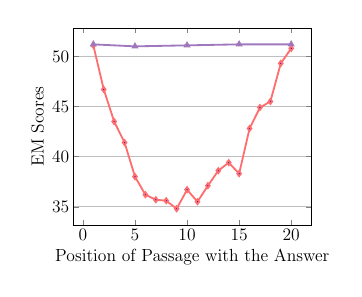
\begin{tikzpicture}[scale=0.44]
    \begin{axis}[
        xlabel=Position of Passage with the Answer,
        ylabel=EM Scores,
        % y label style={at={(-0.00,0.5)}},
        ymajorgrids=true,
        font=\Large,
        legend style={at={(0.5,1.05)},anchor=south,legend columns=3},
        legend cell align={left},
        ]
        \addplot+ [color={rgb,255:red,255;green,110;blue,110},line width=1.5pt,mark=diamond*,mark size=2pt] coordinates {
            (1,51.1)
            (2,46.7)
            (3,43.5)
            (4,41.4)
            (5,38.0)
            (6,36.2)
            (7,35.7)
            (8,35.6)
            (9,34.8)
            (10,36.7)
            (11,35.5)
            (12,37.1)
            (13,38.6)
            (14,39.4)
            (15,38.3)
            (16,42.8)
            (17,44.9)
            (18,45.5)
            (19,49.3)
            (20,50.8)
        };
        \addplot+ [color={rgb,255:red,160;green,120;blue,190},line width=1.5pt,mark=triangle*,mark size=2pt] coordinates {
            (1,51.2)
            (5,51.0)
            (10,51.1)
            (15,51.2)
            (20,51.2)
        };
    \end{axis}
\end{tikzpicture}
\label{fig:answer position}
\end{minipage}
}
\caption{Comparison of LLAMA's and LKG-RALM's performance with retrieved passages.}
\label{fig:LLM challenges}
\end{figure}